
\section{MPS algorithms}

This section, and the following one, will introduce some different tensor network algorithms. The gaol is to provide an intuitive expanation how these algorithm work. For rigorous derivations and mathematical details, other sources can be read.

\subsection{Canonical form}

A translation invariant MPS has the following form:
\begin{equation}\label{mps:uni}
  \pepob{5}{2}{{
        "-","-", "-","-",
        "","","",""}}{{
        "-",
        "",
        "",
        "",
        "-"}}{{
        4,4,4,4,4,
        4,0,0,0,4}}
\end{equation}
It can be easily seen that inserting $X X^{-1}$ on each bond doesn't change the contracted tensor.
\begin{equation}
  A_l = \pepob{3}{2}{{
        "-","-",
        "",""}}{{
        "-",
        "",
        "-"}}{{
        4,4,4,
        4,2,4}}  =X \pepob{3}{2}{{
        "-","-",
        "",""}}{{
        "-",
        "",
        "-"}}{{
        4,4,4,
        4,0,4}} X^{-1}
\end{equation}

\begin{equation}
  A_r = \pepob{3}{2}{{
        "-","-",
        "",""}}{{
        "-",
        "",
        "-"}}{{
        4,4,4,
        4,3,4}}=Y \pepob{3}{2}{{
        "-","-",
        "",""}}{{
        "-",
        "",
        "-"}}{{
        4,4,4,
        4,0,4}} Y^{-1}
\end{equation}
and
\begin{equation}
  \pepob{3}{2}{{
        "-","-",
        "",""}}{{
        "-",
        "-",
        "-"}}{{
        4,4,4,
        4,6,4}}  = X Y^{-1} = C
\end{equation}
Then \cref{mps:uni}  can be written as follows:
\begin{equation}
  \pepob{6}{2}{{
        "-","-", "-","-","-",
        "","","","",""}}{{
        "-",
        "",
        "",
        "-",
        "",
        "-"}}{{
        4,4,4,4,4,4,
        4,2,2,6,3,4}}
\end{equation}
Introducing one more tensor:
\begin{equation}\label{algs:ACC}
  A_c = \pepob{3}{2}{{
        "-","-",
        "",""}}{{
        "-",
        "",
        "-"}}{{
        4,4,4,
        4,7,4}} = \pepob{4}{2}{{
        "-","-", "-",
        "","",""}}{{
        "-",
        "",
        "-",
        "-"}}{{
        4,4,4,4,
        4,2,6,4}} = \pepob{4}{2}{{
        "-","-", "-",
        "","",""}}{{
        "-",
        "-",
        "",
        "-"}}{{
        4,4,4,4,
        4,6,3,4}}
\end{equation}
At the moment the matrices $X$ and $Y$ are not yet defined. To bring an MPS A in its canonical form, the following choice is made

\begin{subequations} \label{algs:mpsid}
  \begin{alignat}{3}
                 & \vcenter{ \hbox{ \pepob{3}{2}{{
              "","",
              "",""}}{{
              "",
              "",
              "-"}}{{
              4,2,4,
    4,2,4}} } }= &                                 & \vcenter{ \hbox{  \pepob{3}{2}{{
              "","-",
              "","-"}}{{
              "",
              "-",
              "-"}}{{
              4,4,4,
    4,4,4}} } }  &                                 & = I                              \\
                 & \vcenter{ \hbox{ \pepob{3}{2}{{
              "","",
              "",""}}{{
              "-",
              "",
              ""}}{{
              4,3,4,
    4,3,4}} } }= &                                 & \vcenter{ \hbox{  \pepob{3}{2}{{
              "","-",
              "","-"}}{{
              "",
              "-",
              "-"}}{{
              4,4,4,
    4,4,4}} } }  &                                 & = I
  \end{alignat}
\end{subequations}

\todo{more on MPS}

\subsubsection{DMRG}

\section{2D tensor network contraction}

PEPS contraction concerns the following problem:
\begin{equation}\label{algs:biggrid}
  \rho_{i,j} =\vcenter{ \hbox{ \pepob{7}{7}{{
            "-","-", "-","-","-","-",
            "",  "", "","","","",
            "",  "", "","","","",
            "",  "", "","","","",
            "",  "", "","","","",
            "",  "", "","","","",
            "-", "-", "-","-","-","-",}}{{
            "-","-", "-","-","-","-",
            "","", "","","","",
            "","", "","","","",
            "","", "","","","",
            "","", "","","","",
            "","", "","","","",
            "-","-", "-","-","-","-",}}{{
            1,13,13,13,13,13,1,
            13,0,0,0,0,0,13,
            13,0,0,0,0,0,13,
            13,0,0,12,0,0,13,
            13,0,0,0,0,0,13,
            13,0,0,0,0,0,13,
            1,13,13,13,13,13,1,
          }} }}
\end{equation}
Contract an infinite lattice of identical tensors, with some irregularities on a small patch. For example, the one patch can be used to calculate an expectation value of a certain observable.

\subsection{Overview methods}

As this is a difficult task, and often the bottleneck in simulations, many algorithms exist to perform this. The classification is taken from \cite{Nietner2020}

\subsubsection{Real-space renormalization-group methods}

The general idea is to course grain the tensor network. Of the many methods, historically the first one was Tensor renormalization group (TRG)  \cite{Hauru}, shown in \cref{fig:tnalgs:trg}. In the first step i, the tensor are split with a SVD in 2 different ways, depending on the position on the lattice. ii recombines 4 halves of the decomposition into 1 new tensor. The result is a rotated grid, with side length $\sqrt{2}$. The bond dimension is truncated during the SVD step.

\begin{figure}
  \center
  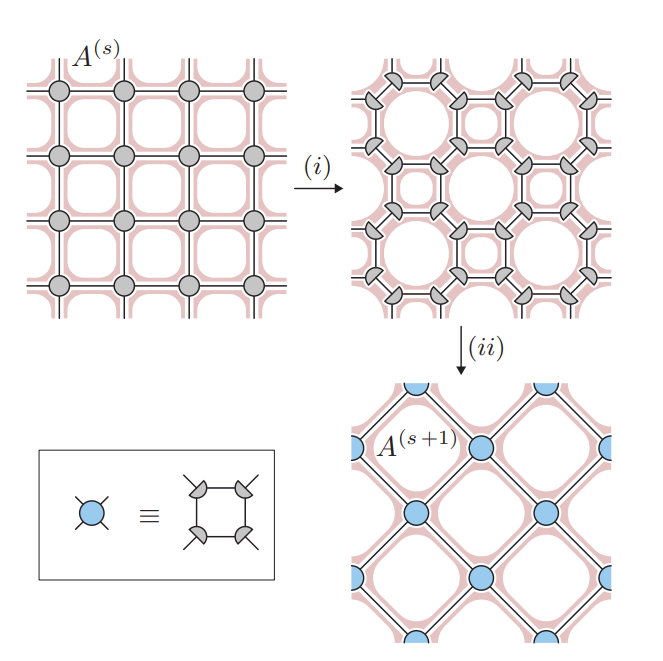
\includegraphics[width=0.5 \textwidth]{Figuren/tnalgs/TRG.png}
  \caption{ Steps in TRG procedure. Figure taken from \cite{Hauru}.  }
  \label{fig:tnalgs:trg}
\end{figure}

Many other variants exist, such as Tensor Network Renormalization (TNR), which wont be discussed here.

\subsubsection{Corner transfer matrix  methods}

Another method goes by the name Corner transfer matrix renormalisation group (CTMRG), as descirbed in \cite{orus}. The full network is approximated by 4 corner matrices and 4 C and 4 half row transfer matrices T as shown in \cref{fig:tnalgs:ctmrg:a}. The idea is to find matrices such that inserting a row and truncating it again results in the same tensors. This is shown in \cref{fig:tnalgs:ctmrg:b}. First, a new row is inserted. From \cref{fig:tnalgs:ctmrg:a} it can be seen that this should not change the environment. Some of the tensors are taken together in step 2. As a final step, the tensor are suitably truncated. Once this cycle converges, the environment is known.

\begin{figure}
  \centering
  \begin{subfigure}[b]{0.8\textwidth}
    \centering
    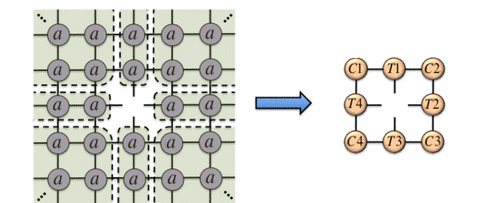
\includegraphics[width=\textwidth]{Figuren/tnalgs/CTMRG_Def.png   }
    \caption{Definition of environment}
    \label{fig:tnalgs:ctmrg:a}
  \end{subfigure}

  \begin{subfigure}[b]{0.7\textwidth}
    \centering
    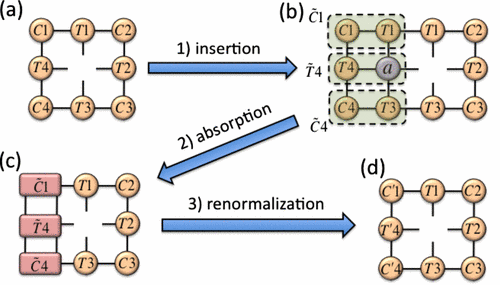
\includegraphics[width=\textwidth]{Figuren/tnalgs/CTMRG.png   }
    \caption{3 steps of CTMRG}
    \label{fig:tnalgs:ctmrg:b}
  \end{subfigure}
  \caption{  Figures adapted from \cite{orus} }
  \label{fig:tnalgs:ctmrg}
\end{figure}

Note that many important details are not written down here, and this is merely to give some intuition about tensor network contraction algorithms.

\subsubsection{Boundary methods}

The goal of these methods is to find an MPS fixed point for the infinite lattice:

\begin{equation}\label{algs:mpslayermpo}
  \pepob{5}{3}{{
        "-","-", "-","-",
        "","","","",
        "","","","",}}{{
        "-", "-",
        "", "",
        "", "",
        "", "",
        "-", "-",}}{{
        4,4,4,4,4,
        13,0,0,0,13,
        13,2,7,3,13}}  \approx  \pepob{5}{2}{{
        "-","-", "-","-",
        "","","",""}}{{
        "-",
        "",
        "",
        "",
        "-"}}{{
        4,4,4,4,4,
        13,2,7,3,13}}
\end{equation}

\paragraph{Time-evolving block decimation }

Time-evolving block decimation was introudec as a method to calculate thermal states (this will also be encountered later on in \cref{para:TEBD}). It can also be used for contraction.

The idea is shown in \cref{fig:tnalgs:tebd}. The boundary MPS is applied, and afterwards trunctued.

\begin{figure}
  \center
  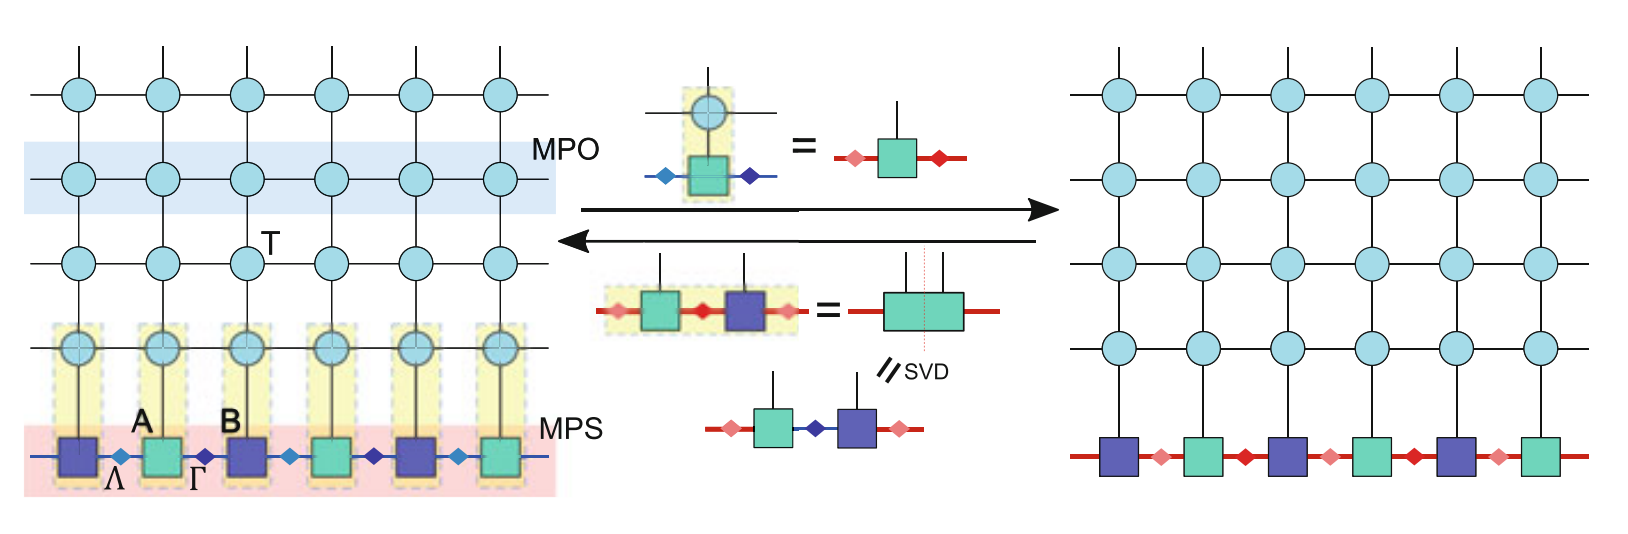
\includegraphics[width=0.5 \textwidth]{Figuren/tnalgs/tn_con_TEBD.png}
  \caption{  Figure taken from \cite{Ran202}.  }
  \label{fig:tnalgs:tebd}
\end{figure}

\todo{update}

\subsection{Vumps}

The purpuse of this section is to give some intuition on the variational uniform Matrix Product State  (VUMPS) algorithm, which will be used later on in this thesis.

The goal is to find a MPS layer for the MPO such that:
\begin{equation}\label{algs:mpslayermpo}
  \pepob{5}{3}{{
        "-","-", "-","-",
        "","","","",
        "","","","",}}{{
        "-", "-",
        "", "",
        "", "",
        "", "",
        "-", "-",}}{{
        4,4,4,4,4,
        13,0,0,0,13,
        13,2,7,3,13}}  \approx  \pepob{5}{2}{{
        "-","-", "-","-",
        "","","",""}}{{
        "-",
        "",
        "",
        "",
        "-"}}{{
        4,4,4,4,4,
        13,2,7,3,13}}
\end{equation}
This is very similar to \cref{algs:exp}. The expression holds approximately, because the MPS on the left hand side has a larger bond dimension than on the right hand side.

\subsubsection{The equations}
Suppose there are tensor which fullfil the conditions stated below:
\begin{subequations} \label{algs:vumpsenv}
  \begin{alignat}{2}
                             & \vcenter{ \hbox{  \pepob{5}{3}{{
              "","-", "-","",
              "","Gl","","",
              "","","",""}}{{
              "-","-",
              "-","-",
              "","",
              "-","-",
              "",""}}{{
              1,4,4,4,1,
              1,4,0,4,1,
    1,5,2,4,1}} }} = \lambda &                                   & \vcenter{ \hbox{    \pepob{5}{3}{{
              "-","-", "-","-",
              "-","","Gl","-",
              "-","","","-"}}{{
              "-","-",
              "-","-",
              "","",
              "-","-",
              "-","-"}}{{
              1,4,4,4,1,
              1,4,2,4,1,
    1,1,5,4,1}}}}                                                                                     \\
                             & \vcenter{ \hbox{   \pepob{5}{3}{{
              "-","-", "-","-",
              "","","Gr","-",
              "","","",""}}{{
              "-","-",
              "-","-",
              "","",
              "-","-",
              "-","-"}}{{
              1,4,4,4,1,
              1,4,0,4,1,
    1,4,8,1,1}} }}=  \lambda &                                   & \vcenter{ \hbox{ \pepob{5}{3}{{
              "-","-", "-","-",
              "-","-","Gr","",
              "-","-","",""}}{{
              "-","-",
              "-","-",
              "-","-",
              "","",
              "-","-"}}{{
              1,1,4,4,4,
              1,1,4,3,4,
              1,1,10,1,1}} }}
  \end{alignat}
\end{subequations}

These eigentensor equations are solved in pratice in a slightly different manner:
\begin{equation}\label{vumps_transfer_eigs}
  \vcenter{ \hbox{   \pepob{5}{3}{{
            "-","", "","-",
            "","","Gr","-",
            "","","",""}}{{
            "-","-",
            "-","-",
            "","",
            "","",
            "-","-"}}{{
            1,4,3,4,1,
            1,4,0,4,1,
            1,4,8,1,1}} }}=  \lambda  \vcenter{ \hbox{ \pepob{5}{3}{{
            "-","", "","",
            "-","-","Gr","",
            "-","-","",""}}{{
            "-","-",
            "-","-",
            "-","-",
            "","",
            "",""}}{{
            1,1,4,4,1,
            1,1,4,4,1,
            1,1,10,1,1}} }}
\end{equation}
Wher the $ Ar  $ tensor was connected from below on both sides and \cref{algs:mpsid} was used on the right hand side. The blocks in \cref{algs:vumpsenv} form a zipper from the left and right respectively. Each application brings down one of the MPS tensors in the following way.
\begin{equation}
  \begin{split}
    &       \vcenter{ \hbox{ \pepob{7}{3}{{
              "-","-", "-","-","-","-",
              "","Gl","","","","",
              "","","","","","",}}{{
              "-", "-",
              "", "",
              "", "",
              "", "",
              "", "",
              "", "",
              "-", "-",}}{{
              1,4,4,4,4,4,4,
              13,2,0,0,0,0,13,
              1,5,2,2,2,2,13}}}} \\
    =&       \vcenter{ \hbox{ \pepob{7}{3}{{
              "-","-", "-","-","-","-",
              "","","Gl","","","",
              "","","","","","",}}{{
              "-", "-",
              "", "",
              "", "",
              "", "",
              "", "",
              "", "",
              "-", "-",}}{{
              1,4,4,4,4,4,4,
              13,2,2,0,0,0,13,
              1,1,5,2,2,2,13}}}} \\
    =&       \vcenter{ \hbox{ \pepob{7}{3}{{
              "-","-", "-","-","-","-",
              "","","","Gl","","",
              "","","","","","",}}{{
              "-", "-",
              "", "",
              "", "",
              "", "",
              "", "",
              "", "",
              "-", "-",}}{{
              1,4,4,4,4,4,4,
              13,2,2,2,0,0,13,
              1,1,1,5,2,2,13}}}} \\
  \end{split}
\end{equation}
The left and right zipper can now move towards each other, until they meet at the center. In order to become the same MPS as before the application to the MPO (\cref{algs:mpslayermpo}), one more condition is needed:
\begin{equation} \label{algs:AC}
  \vcenter{ \hbox{   \pepob{5}{3}{{
            "-","-", "-","-",
            "","Gl","Gr","-",
            "","","",""}}{{
            "-","-",
            "-","-",
            "","",
            "-","-",
            "-","-"}}{{
            1,4,4,4,1,
            1,4,0,4,1,
            1,5,9,1,1}} }}=  \lambda  \pepob{3}{2}{{
        "-","-",
        "",""}}{{
        "-",
        "",
        "-"}}{{
        4,4,4,
        4,7,4}}
\end{equation}
This completely determines the problem, but one more equation is used to solve the problem. Combining on of the equations \cref{algs:vumpsenv}, the definitipn of $A_c$ \cref{algs:AC} and one of \cref{algs:mpsid} gives $C$:
\begin{equation}\label{algs:vumpsenvc}
  \vcenter{ \hbox{   \pepob{5}{3}{{
            "-","-", "-","-",
            "","Gl","Gr","-",
            "","","",""}}{{
            "-","-",
            "-","-",
            "-","-",
            "-","-",
            "-","-"}}{{
            1,4,4,4,1,
            1,4,4,4,1,
            1,5,11,1,1}} }}  =  \lambda  \pepob{3}{2}{{
        "-","-",
        "",""}}{{
        "-",
        "-",
        "-"}}{{
        4,4,4,
        4,6,4}}
\end{equation}
\todo{fix gap}

Then  \cref{algs:mpslayermpo} is solved:

\begin{equation}
  \begin{split}
    & \vcenter{ \hbox{ \pepob{7}{3}{{
              "-","-", "-","-","-","-",
              "","","","","","",
              "","","","","","",}}{{
              "-", "-",
              "", "",
              "", "",
              "", "",
              "", "",
              "", "",
              "-", "-",}}{{
              4,4,4,4,4,4,4,
              13,0,0,0,0,0,13,
              13,2,2,7,3,3,13}} }}\\
    &=       \vcenter{ \hbox{ \pepob{7}{3}{{
              "-","-", "-","-","-","-",
              "","Gl","","","Gr","",
              "","","","","","",}}{{
              "-", "-",
              "", "",
              "", "",
              "", "",
              "", "",
              "", "",
              "-", "-",}}{{
              1,4,4,4,4,4,4,
              13,2,0,0,0,3,13,
              1,5,2,7,8,1,4}}}} \\
    &=  \vcenter{ \hbox{ \pepob{7}{3}{{
              "-","-", "-","-","-","-",
              "","","Gl","Gr","","",
              "","","","","","",}}{{
              "-", "-",
              "", "",
              "", "",
              "", "",
              "", "",
              "", "",
              "-", "-",}}{{
              1,4,4,4,4,4,4,
              13,2,2,0,3,3,13,
              1,1,5,9,1,1,1}} }}\\
    &= \vcenter{ \hbox{ \pepob{7}{3}{{
              "-","-", "-","-","-","-",
              "","","","","","",
              "","","","","","",}}{{
              "-", "-",
              "", "",
              "", "",
              "", "",
              "", "",
              "", "",
              "-", "-",}}{{
              1,4,4,4,4,4,4,
              13,2,2,7,3,3,13,
              1,1,1,1,1,1,1}} }}
  \end{split}
\end{equation}

\todo{check lambdas in literature}

Contracting a 2D tensor network is thus reduced to solving the  \cref{algs:ACC}, \cref{algs:vumpsenv}, \cref{algs:AC} and \cref{algs:vumpsenvc} simultaneously. Inspection of the equations show that the following cycle needs to be solved:

\begin{itemize}
  \item  $A_c,C  \rightarrow A_l,A_r  $  \cref{algs:ACC}
  \item  $A_l,A_r  \rightarrow G_l,G_r  $ \cref{algs:vumpsenv}
  \item  $ G_l,G_r   \rightarrow Ac,C $ \cref{algs:AC} and  \cref{algs:vumpsenvc}
\end{itemize}

The calculated environment can now be used to solve the original problem. Due to symmetry, the same MPS can be applied from below. \cref{algs:vumpsenvc} now becomes:
\begin{equation}
  \vcenter{ \hbox{   \pepob{5}{3}{{
            "","", "","",
            "","Gl","Gr","",
            "","","",""}}{{
            "-","-",
            "","",
            "","",
            "","",
            "-","-"}}{{
            13,2,7,3,13,
            13,2,4,3,13,
            1,5,9,1,1}} }}
\end{equation}

\subsubsection{The derivation}\label{vumps_Deriv}
While the above derivation is reasonable, it is not very rigorous. The algorithm finds its origins  in tangent space methods, such as explained in \cite{Vanderstraeten2019}.

Not every state in the many body Hillbert space can be represented by an MPS. For a

By carefully constructing the tangent space and making use of the available gauge freedom, a compact expression can be found for the tangent space projector $\mathcal{P}_A$. This projects a state from the many body Hillbert space to the tangent space of an MPS A. For an optimal MPS approximation A, the error made in the approximation should be orthogonal to the tangent space. For \cref{algs:mpslayermpo} this means that the application of the projection of the error on the tangent space should be zero, i.e. the MPS is at a variational minimum.  \cite{Nietner2020}

Applying the projector $\mathcal{P}_A$ to \cref{algs:mpslayermpo} exactly gives rise to the equations stated earlier.

